\documentclass[lettersize,journal]{IEEEtran}
\usepackage{amsmath,amsfonts}
\usepackage{algorithmic}
\usepackage{algorithm}
\usepackage{array}
\usepackage[caption=false,font=normalsize,labelfont=sf,textfont=sf]{subfig}
\usepackage{textcomp}
\usepackage{stfloats}
\usepackage{url}
\usepackage{verbatim}
\usepackage{graphicx}
\usepackage{cite}
\usepackage{tikz}
\usepackage{verbatim}
\usetikzlibrary{mindmap,trees}
\hyphenation{op-tical net-works semi-conduc-tor IEEE-Xplore}

\begin{document}

\title{Data-Driven Autonomous Driving Simulation: Survey}
\author{Jayesh Choudhary and Arhan Vora}
\date{17 September 2024}

\maketitle

\begin{abstract}
The Data Driven Autonomous Driving Simulation plays a significant role in development of Autonomous driving as real world testing of autonomous vehicles is very expensive as well as dangerous which presents technical and safety threats along with regulatory challenges.The data driven autonomous driving simulation helps greatly in reducing the expense and safely test and validate the vehicles and thus refine the autonomous vehicles for better and faster growth fulfilling its purpose. 

A major problem in advancement of autonomous driving is the upper bound of autonomous driving algorithm's performance, especially in handling extreme and complex driving scenarios due to lack of real world data for such conditions as well as the lack of detailing in the data for such critical cases since the data is generally collected only from cameras instead of using the data from various sensors. The key to overcome this upper bound lies in the data-centric autonomous driving technologies which emphasises the importance of high quality data for diverse conditions in optimizing current algorithms and collecting and utilizing autonomous driving data along with dynamically upgrading it.
The recent advancement in AD simulation, closed loop model training and the increase in data has been a valuable experience. However, the lack of systematic knowledge and deep understanding regarding how to built efficient data-centric autonomous driving technology are still major research gaps.

In this project we understand the state of data-driven autonomous driving simulation and how core technologies like artificial intelligence, machine learning, deep neural networks, sensor data fusion, synthetic data generation for rare but critical cases, integration of real-time data processing capabilities through 5G and edge computing contribute to the growth of autonomous vehicles' performance.

\end{abstract}

\begin{IEEEkeywords}
Data-Driven Autonomous Driving Simulation, Real-World Testing Challenges, Sensor Data Fusion, Synthetic Data Generation, Closed-Loop Model Training, Autonomous Driving Data Collection, Performance Optimization for Self-Driving Cars, Autonomous Driving Algorithms, Simulation-Based Validation, Autonomous Driving Safety
\end{IEEEkeywords}

\section{introduction}
\IEEEPARstart{A}{utonomous} vehicles (AVs) have become a major focus in research, thanks to its potential of revolutionizing transportation and enhancing road safety \cite{janai2020computer}.One of the most transformative and rapidly growing technologies of the 21st century in the transportation sector is represented by autonomous driving \cite{mirzai2023future}. However, real world on road testing for autonomous vehicles still remains a challenge due to its high costs \cite{NEURIPS2023_1838feeb} , safety issues, scalability, and coverage of rare edge case scenarios. In addition, regulatory hurdles add to the complexity of real-world testing. Moreover, regulatory hurdles add another layer of complexity to real-world experimentation. Data-driven simulation has hence emerged as an indispensible tool to progress the development of autonomous vehicle technology in a safer, more scalable, and cost-effective fashion to develop and validate the system.

Autonomous driving systems are extremely complex by bringing a massive amount of technological surroundings that include sensing, localization, perception, and decision making \cite{liu2017computer}. In addition, the application relies absolutely on the seamless interaction, which needs to happen between cloud platforms, huge data storages, and HD maps \cite{liu2017computer}.

Though promising, autodriving technology faces a major performance hurdle given the current limitations of algorithms and the complexity of real-world driving conditions  \cite{li2023datacentric}. Data-driven simulation relies on the vast amount of real-world driving data from cameras, sensor inputs, artificial intelligence, machine learning models to create highly realistic virtual environments. These simulations allow developers to test autonomous driving in a vast variety of scenarios- like heavy traffic, rare conditions like natural disasters, extreme weather conditions, interaction with erratic drivers- which are difficult to test in real world. By improving algorithms in a controlled virtual environment, developers can enhance the performance of autonomous vehicle systems while reducing the danger and expense.

One of the major obstacles in the growth of AVs is the limitation of real world data, especially for rare and extreme driving situations.  90\% of the autonomous driving data received is for normal driving scenarios \cite{ref1}. Autonomous vehicles lack sufficient data to train their models for critical cases that do not occur often. These unusual, however critical scenarios help in training AV models to deal with the unexpected situation so that self-driving systems are secure and more reliable. In the event of an encounter with too few exposures towards these edge cases, AVs may fail to properly react at critical times.
This issue is further complicated by the fact that most of training data is from lesser variety of sensors, particularly cameras leaving out essential information from other sensors \cite{ref1}. This lack of diverse sensor data leaves gaps in spatial understanding and reduces the robustness of AV systems when complex driving conditions arise in front of them. Overcoming these limitations requires more data from extreme driving scenarios and the integration of multi-sensor data to form a basis for more resilient and adaptable autonomous systems.

Later progresses in high-fidelity test systems presently make it conceivable to prepare independent driving operators in closed circle, possibly circumventing inside and out the unmanageable issue of how to control the conveyance move that arises between training and deployment, and enabling scaling of training both safely and very cheaply. There is relatively little known about how to build benchmarking aids to train in closed-loop settings. \cite{zhang2022rethinking}.

Our research focuses on the use of next generation technologies to improve and develop data-driven autonomous driving simulators, with a focus on advanced machine learning techniques in sensor fusion and on-generation synthetic data for some of the very rarest or most hazardous scenarios. Synthetic data, as such, is useful to create realistic simulations of challenging conditions that would be hard or impossible to replicate in real world experiments. Such simulation enables training in a well-controlled, safe environment and therefore increases the robustness and reliability of autonomous systems.

Emerging trends further enrich this landscape of simulations. As 5G and edge computing start to come into the picture for real-time processing, simulation fidelity, as well as the responsiveness of simulations, has been taken to new heights - enable a machine system to process and answer information more quickly and accurately. Human-AI collaboration is moreover of tall significance, since human-in-the-loop frameworks reveal imperative disclosures on intelligent between independent and human drivers to move forward more secure and more agreeable driving situations.

This development, however comes with huge challenges: knowledge and models developed in simulation must be successfully transferred to real applications. This will call for techniques like domain adaptation and generalization to ensure efficient bridging between virtual and real-world performances. There is also a need to bring to the fore the regulatory standards of simulation frameworks, which change over time, along with critical ethical questions such as fairness, bias reduction, and accountability within AI decision-making.


\begin{figure}[h]
    \centering
    \resizebox{\linewidth}{!}{ % Resizes the image to fit within the text width
    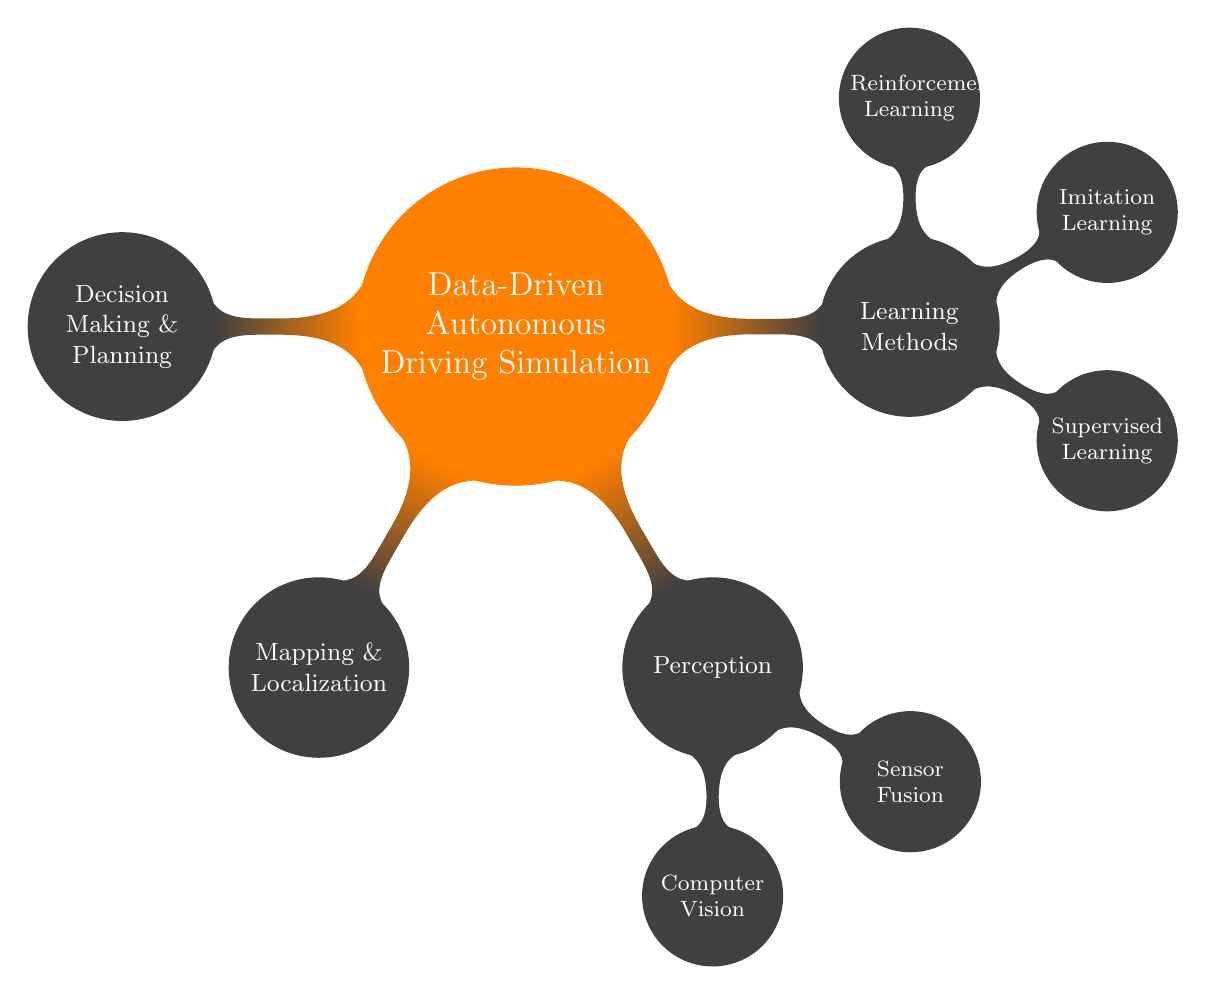
\begin{tikzpicture}
      \path[mindmap,concept color=orange,text=white]
        node[concept] {Data-Driven Autonomous\\Driving Simulation}
        [clockwise from=0]
        child[concept color=gray!50!black] {
          node[concept] {Learning Methods}
          [clockwise from=90]
          child { node[concept] {Reinforcement Learning} }
          child { node[concept] {Imitation Learning} }
          child { node[concept] {Supervised Learning} }
        }  
        child[concept color=gray!50!black] {
          node[concept] {Perception}
          [clockwise from=-30]
          child { node[concept] {Sensor Fusion} }
          child { node[concept] {Computer Vision} }
        }
        child[concept color=gray!50!black] { node[concept] {Mapping \& Localization} }
        child[concept color=gray!50!black] { node[concept] {Decision Making \& Planning} };
    \end{tikzpicture}
    }
    \caption{Mind map of data-driven autonomous driving simulation technologies.}
    \label{fig:mindmap}
\end{figure}

\section{Literature Search and Selection}
\subsection{Search Strategy}
\subsubsection{Sources and Databases}
We have used sources, including Google Scholar, IEEE Xplore, ScienceDirect, CiteSeerX, ACM Digital Library, and SpringerLink. These have many quality research papers presented in the top conference across the globe and, hence, have proven to be excellent resources for this project.

\subsubsection{GitHub}
Papers have also been cross-referenced from GitHub repositories such as Awesome Data Centric Autonomous Driving by LincanLi98, End-to-End Autonomous Driving from OpenDriveLab, and related papers from the page on SafeAV's GitHub page.

\subsubsection{Search Terms}
The keywords used to filter the search results include:
\begin{itemize}
    \item Autonomous Driving
    \item Autonomous Driving Simulations
    \item Data-Driven Driving Simulations
    \item ML-based Driving
    \item Intelligent Driving Systems
    \item Algorithms for Autonomous Driving
\end{itemize}

\subsubsection{Time Frame}
Our focus was on papers published in the last decade, specifically from 2014 to 2024.

\subsection{Inclusion Criteria}
\subsubsection{Relevance}
We are in this study to bring on board research aimed at addressing the use of different machine learning models and algorithms towards achieving autonomous driving systems. Again, the paper should share information on improving efficiency through data training on the models while the testing phase rotates around the simulations used to analyze their performance.

\subsubsection{Quality}
 The articles should have huge impact and applications on real world research-projects. Refer from sources which have gone through rigorous reviewing and have been validated by experts in the field.

\subsubsection{Publication Type}
Only quality research papers and published articles that have been accepted and passed through peer review by experts in the same field are used. Also, conference papers, conclusions from reliable and trustworthy sources, and technical reports that have been verified also come within this category.

\subsection{Exclusion Criteria}
\subsubsection{Irrelevance}
Studies which do not focus on Data Driven Autonomous Driving Simulation, it's application or reviews. The study should be aligned with the central theme of our review. Articles without a clear connection to our topic of research and those without any clear conclusion or insights should be excluded.

\subsubsection{Quality}
Exclude studies which are controversial, have proven flaws, have low credibility, showcase insufficient data. Papers which have an unclear focus, questionable assumptions, bad design, unprofessional content should be excluded.

\subsubsection{Publication Type}
Articles published by sources that are not trustworthy, non-technical publishers, articles that have not been reviewed, opinions, and incomplete research results were not be included.

\subsection{Screening}
We started screening for study selection by searching the mentioned keywords across multiple research databases.
Then we proceeded to screen them on basis of the relevance to the topic and credibility scores. We filtered out 
the papers which were irrelevant to our topic and those which had low credibility. Next we filtered out those which
did not prove to be up to the quality standards set by us as described above. We then started to go through these 
research papers and started extracting the information from these selected sources and integrated them into our own
survey report providing appropriate references and citations.
This approach guaranteed that we not only covered a wide range of diverse studies on the topic but also covered the
topic in depth allowing us to present an in-depth comprehensive analysis report for the wide range of topics included.
As a result we not only covered the breadth of the subject but also reached an appropriate depth in the subject.

\section{Simple References}

\begin{thebibliography}{1}
\bibliographystyle{IEEEtran}

\bibitem{janai2020computer}
Joel Janai, Fatma G{\"u}ney, Aseem Behl, Andreas Geiger,
\textit{Computer vision for autonomous vehicles: Problems, datasets and state of the art},
Foundations and Trends{\textregistered} in Computer Graphics and Vision, 
vol. 12, no. 1--3, pp. 1--308, 2020.

\bibitem{mirzai2023future}
Sabiq Mirzai.
\newblock The Future of Autonomous Vehicles: Revolutionizing Transportation and Society.
\newblock \emph{TechCrate}, May 24, 2023.
\newblock \url{https://techcrate.com/the-future-of-autonomous-vehicles-revolutionizing-transportation-and-society}.


\bibitem{NEURIPS2023_1838feeb}
Cole Gulino, Justin Fu, Wenjie Luo, George Tucker, Eli Bronstein, Yiren Lu, Jean Harb, Xinlei Pan, Yan Wang, Xiangyu Chen, John Co-Reyes, Rishabh Agarwal, Rebecca Roelofs, Yao Lu, Nico Montali, Paul Mougin, Zoey Yang, Brandyn White, Aleksandra Faust, Rowan McAllister, Dragomir Anguelov, and Benjamin Sapp.
\newblock Waymax: An Accelerated, Data-Driven Simulator for Large-Scale Autonomous Driving Research.
\newblock In \emph{Advances in Neural Information Processing Systems}, volume 36, pages 7730--7742, 2023.
\newblock Curran Associates, Inc.
\newblock \url{https://proceedings.neurips.cc/paper_files/paper/2023/file/1838feeb71c4b4ea524d0df2f7074245-Paper-Datasets_and_Benchmarks.pdf}.

\bibitem{li2023datacentric}
Lincan Li, Wei Shao, Wei Dong, Yijun Tian, Qiming Zhang, Kaixiang Yang, Wenjie Zhang, 
"Data-Centric Evolution in Autonomous Driving: A Comprehensive Survey of Big Data System, Data Mining, and Closed-Loop Technologies," 
Data and Knowledge Research Group, University of New South Wales, Sydney, Australia, 2023.


\bibitem{liu2017computer}
S. Liu, J. Peng, and J.-L. Gaudiot, "Computer drive my car!", \textit{Computer}, vol. 50, no. 1, pp. 8, 2017.

\bibitem{ref1}
Lincan Li, \textit{Awesome Data-Centric Autonomous Driving}, Available at: \url{https://github.com/LincanLi98/Awesome-Data-Centric-Autonomous-Driving}, Accessed: September 2024.

\bibitem{ref2}
R. Zong, W. Deng, X. Bai, Y. Wang, and J. Ding, ``Traffic Modeling Based on Data-Driven Method for Simulation Test of Autonomous Driving,'' \textit{IEEE Transactions on Intelligent Transportation Systems}, vol. 24, no. 12, pp. 14076-14085, 2023. doi: 10.1109/TITS.2023.3304972.

\bibitem{ref3}
A. Amini, I. Gilitschenski, J. Phillips, J. Moseyko, R. Banerjee, S. Karaman, and D. Rus, ``Learning Robust Control Policies for End-to-End Autonomous Driving From Data-Driven Simulation,'' \textit{IEEE Robotics and Automation Letters}, vol. 5, no. 2, pp. 1143-1150, 2020. doi: 10.1109/LRA.2020.2966414.

\bibitem{ref4}
C. Gulino, J. Fu, W. Luo, G. Tucker, E. Bronstein, Y. Lu, J. Harb, X. Pan, Y. Wang, X. Chen, J. Co-Reyes, R. Agarwal, R. Roelofs, Y. Lu, N. Montali, P. Mougin, Z. Yang, B. White, A. Faust, R. McAllister, D. Anguelov, and B. Sapp, ``Waymax: An Accelerated, Data-Driven Simulator for Large-Scale Autonomous Driving Research,'' in \textit{Advances in Neural Information Processing Systems}, vol. 36, A. Oh, T. Naumann, A. Globerson, K. Saenko, M. Hardt, and S. Levine, Eds., Curran Associates, Inc., 2023, pp. 7730--7742. Available: \url{https://proceedings.neurips.cc/paper_files/paper/2023/file/1838feeb71c4b4ea524d0df2f7074245-Paper-Datasets_and_Benchmarks.pdf}.

\bibitem{ref5}
T.-H. Wang, A. Amini, W. Schwarting, I. Gilitschenski, S. Karaman, and D. Rus, ``Learning Interactive Driving Policies via Data-driven Simulation,'' in \textit{Proceedings of the 2022 International Conference on Robotics and Automation (ICRA)}, pp. 7745-7752, 2022. doi: 10.1109/ICRA46639.2022.9812407.

\bibitem{ref6}
F. Mütsch, H. Gremmelmaier, N. Becker, D. Bogdoll, M. R. Zofka, and J. M. Zöllner, ``From Model-Based to Data-Driven Simulation: Challenges and Trends in Autonomous Driving,'' arXiv preprint arXiv:2305.13960, 2023. Available: \url{https://arxiv.org/abs/2305.13960}.

\bibitem{ref7}
T.-H. Wang, A. Amini, W. Schwarting, I. Gilitschenski, S. Karaman, and D. Rus, ``Learning Interactive Driving Policies via Data-driven Simulation,'' in \textit{Proceedings of the 2022 International Conference on Robotics and Automation (ICRA)}, 2022, pp. 7745-7752. doi: \url{10.1109/ICRA46639.2022.9812407}.

\bibitem{ref8}
R. Zong, W. Deng, X. Bai, Y. Wang, and J. Ding, ``Traffic Modeling Based on Data-Driven Method for Simulation Test of Autonomous Driving,'' \textit{IEEE Transactions on Intelligent Transportation Systems}, vol. 24, no. 12, pp. 14076-14085, 2023. doi: \url{10.1109/TITS.2023.3304972}.

\bibitem{ref9}
D. Dauner, M. Hallgarten, T. Li, X. Weng, Z. Huang, Z. Yang, H. Li, I. Gilitschenski, B. Ivanovic, M. Pavone, A. Geiger, and K. Chitta, ``NAVSIM: Data-Driven Non-Reactive Autonomous Vehicle Simulation and Benchmarking,'' 2024. [Online]. Available: \url{https://arxiv.org/abs/2406.15349}.

\bibitem{ref10}
D. Zhao, Y. Liu, C. Zhang, and Y. Li, ``Autonomous Driving Simulation for Unmanned Vehicles,'' in \textit{2015 IEEE Winter Conference on Applications of Computer Vision}, 2015, pp. 185-190. doi: 10.1109/WACV.2015.32.

\bibitem{ref11}
B. Osiński, A. Jakubowski, P. Zięcina, P. Miłoś, C. Galias, S. Homoceanu, and H. Michalewski, ``Simulation-Based Reinforcement Learning for Real-World Autonomous Driving,'' in \textit{2020 IEEE International Conference on Robotics and Automation (ICRA)}, 2020, pp. 6411-6418. doi: 10.1109/ICRA40945.2020.9196730.

\bibitem{zhang2022rethinking}
Chris Zhang, Runsheng Guo, Wenyuan Zeng, Yuwen Xiong, Binbin Dai, Rui Hu, Mengye Ren, Raquel Urtasun,
\textit{Rethinking Closed-Loop Training for Autonomous Driving}, in \textit{Proceedings of the European Conference on Computer Vision}, Springer, 2022, pp. 264--282.


\end{thebibliography}


\end{document}
